% -----------------------------------------------
% Template for SMC 2022
% based on SMC 2022 template
% -----------------------------------------------

\documentclass{article}

\usepackage{smc}
\usepackage{times}
\usepackage{ifpdf}
\usepackage[english]{babel}
\usepackage{cite}
\usepackage[dvipsnames]{xcolor}
\def\TLcomment[#1]{\textcolor{red}{#1}}
\def\SWcomment[#1]{\textcolor{blue}{#1}}
\def\SScomment[#1]{\textcolor{orange}{#1}}

%%%%%%%%%%%%%%%%%%%%%%%% Some useful packages %%%%%%%%%%%%%%%%%%%%%%%%%%%%%%%
%%%%%%%%%%%%%%%%%%%%%%%% See related documentation %%%%%%%%%%%%%%%%%%%%%%%%%%
\usepackage{amsmath} % popular packages from Am. Math. Soc. Please use the 
\usepackage{amssymb} % related math environments (split, subequation, cases,
\usepackage{amsfonts}% multline, etc.)
%\usepackage{bm}      % Bold Math package, defines the command \bf{}
%\usepackage{paralist}% extended list environments
%%subfig.sty is the modern replacement for subfigure.sty. However, subfig.sty 
%%requires and automatically loads caption.sty which overrides class handling 
%%of captions. To prevent this problem, preload caption.sty with caption=false 
%\usepackage[caption=false]{caption}
%\usepackage[font=footnotesize]{subfig}

\def\ctxt{\text{c}} %connection subscript (text)
\def\stxt{{\text{s}}} %string subscript (text)
\def\ptxt{\text{p}} %plate subscript (text)
\def\mtxt{\text{m}} %mass subscript (text)
\def\itxt{\text{i}} %point of 'interest' subscript (text)
\def\Btxt{\text{B}} %bow subscript (text)
\def\etxt{\text{e}} %excitation subscript (text)
\def\rtxt{\text{r}} %lip reed subscript (text)
\def\ttxt{\text{t}} %tube subscript (text)


\def\sgn{\text{sgn}}
\def\sm{\text{sm}} %string-mass interaction tromba
\def\mp{\text{mp}} %mass-plate interaction tromba

\def\MoneD{{\mathcal{M}^n}}
\def\MtwoD{{\mathcal{M}_2^n}}

\def\Nfrac{\mathcal{N}}
\def\flip{\leftarrow}
\def\Ucal{\mathbfcal{U}}

% states
\def\uln{u_l^n}
\def\wln{w_l^n}
\def\wmn{w_m^n}
\def\un{u^n}
\def\ulmn{u_{l,m}^n}
\def\ulm{u_{l,m}}
\def\uqn{u_q^n}
\def\qlmn{q_{l,m}^n}

\def\wlmn{w_{l,m}^n}
\def\zlmn{z_{l,m}^n}
\def\ubr{u_\text{br}}
\def\zbr{z_\text{br}}

\def\qln{q_l^n}
\def\lv{{l_v}}
\def\lw{{l_w}}
\def\vlvn{v_\lv^n}
\def\ulcn{u_{l_\ctxt}^n}
\def\wlwn{w_\lw^n}
\def\wmcn{w_{m_\ctxt}^n}

\def\wmn{w_m^n}

\def\Psiln{\Psi_l^n}
\def\Psinp{\Psi_l^{n+1}}
\def\Psinm{\Psi_l^{n-1}}
\def\Psilp{\Psi_{l+1}^n}
\def\Psilm{\Psi_{l-1}^n}

% bold symbols (state vectors and matrices)
\def\u{\mathbf{u}}
\def\w{\mathbf{w}}
\def\ww{\boldsymbol{w}}
\def\q{\mathbf{q}}
\def\v{\mathbf{v}}
\def\vv{\boldsymbol{v}}
\def\z{\mathbf{z}}
\def\Z{\mathbf{Z}}
\def\I{\mathbf{I}}
\def\A{\mathbf{A}}
\def\B{\mathbf{B}}
\def\C{\mathbf{C}}
\def\Q{\mathbf{Q}}
\def\U{\mathbf{U}}
\def\J{\mathbf{J}}
\def\i{\mathbf{i}}
\def\j{\mathbf{j}}
\def\BB{\mathbfcal{B}^n}


% interpolators
\def\Iu{I_{l, u}(x_\ctxt)}
\def\Iw{I_{m, w}(\chi_\ctxt)}
\def\Ju{J_{l, u}(x_\ctxt)}
\def\Jw{J_{m, w}(\chi_\ctxt)}
\def\Iq{I_q(\chi_\ctxt)}
\def\Ilm{I_{l,m}(x_\ctxt)}

\def\uStack{\boldsymbol{u}}
\def\qq{\boldsymbol{q}}

% mathfraks
\def\H{\mathfrak{H}}
\def\h{\mathfrak{h}}
\def\t{\mathfrak{t}}
\def\b{\mathfrak{b}}
\def\p{\mathfrak{p}}
% continuous operators
\def\ptt{\partial_t^2} 
\def\pxx{\partial_x^2}
\def\pxxx{\partial_x^3}
\def\pxxxx{\partial_x^4}
\def\pcc{\partial_{\chi}^2}
\def\pcccc{\partial_{\chi}^4}

\def\pyy{\partial_y^2}

\def\pt{\partial_t} 
\def\px{\partial_x} 
\def\py{\partial_y} 

% discrete operators
\def\dtt{\delta_{tt}} 
\def\dxx{\delta_{xx}}
\def\dxxx{\delta_{xxx}}
\def\dxxxx{\delta_{xxxx}}
\def\dcc{\delta_{\chi\chi}}
\def\dcccc{\delta_{\chi\chi\chi\chi}}

\def\dtd{\delta_{t\cdot}} 
\def\dtp{\delta_{t+}} 
\def\dtm{\delta_{t-}} 

\def\dxd{\delta_{x\cdot}} 
\def\dxp{\delta_{x+}} 
\def\dxm{\delta_{x-}} 
\def\dyd{\delta_{y\cdot}} 
\def\dyp{\delta_{y+}} 
\def\dym{\delta_{y-}} 

\def\mtt{\mu_{tt}} 
\def\mtd{\mu_{t\cdot}} 
\def\mtp{\mu_{t+}} 
\def\mtm{\mu_{t-}} 

\def\mxx{\mu_{xx}} 
\def\mxd{\mu_{x\cdot}} 
\def\mxp{\mu_{x+}} 
\def\mxm{\mu_{x-}} 

\def\dDelta{\delta_{\Delta}}
% \def\dDbox{\delta_{\Delta\boxplus}}
\def\dyy{\delta_{yy}}

% matrix operators
\def\Dxx{\mathbf{D}_{xx}}
\def\Dyy{\mathbf{D}_{yy}}
\def\DDxx{\mathbfcal{D}_{xx}^n}
\def\DDyy{\mathbfcal{D}_{yy}^n}
\def\Dxxxx{\mathbf{D}_{xxxx}}
\def\DDxxxx{\mathbfcal{D}_{xxxx}^n}

\def\DDeltamat{\mathbf{D}_\Delta}
\def\DDeltaDelta{\mathbf{D}_{\Delta\Delta}}
\def\DDDelta{\mathbfcal{D}_{\Delta}^n}
\def\DDDeltaDelta{\mathbfcal{D}_{\Delta\Delta}^n}

\def\Mv{M_v^n}
\def\Mw{M_w^n}

% often-used variables
\def\sz{\sigma_{0}}
\def\so{\sigma_{1}}
\def\vrel{v_\text{rel}}
\def\Sbar{\bar{S}}
\def\Sm{S_{l-1/2}}
\def\Sp{S_{l+1/2}}

\def\szX[#1]{\sigma_{0,{#1}}}
\def\soX[#1]{\sigma_{1,{#1}}}

\def\fs{f_\text{s}}
\def\el{\epsilon_\text{l}}
\def\er{\epsilon_\text{r}}
% mathcals
\def\D{\mathcal{D}}
\def\L{\mathcal{L}}
\def\OO{\mathcal{O}}
\def\S{\mathcal{S}}

% flooring ceiling
\def\floor[#1]{\left\lfloor #1 \right\rfloor}
\def\ceil[#1]{\left\lceil #1 \right\rceil}
\def\ansatz{\ \overset{\mathcal{A}}{\Longrightarrow}\ }
% other
\def\qaq{\quad \text{and} \quad}
\def\qwiq{\quad \text{with} \quad}
\def\qwhq{\quad \text{where} \quad}

\def\mystrut{\rule[-.2\baselineskip]{0pt}{\baselineskip}}

\def\th{\textsuperscript{th} }
\def\thOrder{\textsuperscript{th}-order }

\def\boldPhi{\boldsymbol{\phi}}
\def\boldPsi{\boldsymbol{\Psi}}
\def\eig{\text{eig}}

\def\Dxx{\mathbf{D}_{xx}}
\def\alf{'}
\def\DxxA{\Dxx\alf}
\def\DyyA{\Dyy\alf}
\def\DxxxxA{\Dxxxx\alf}
\def\DDeltamatA{\DDeltamat\alf}
\def\DDeltaDeltaA{\DDeltaDelta\alf}
\def\Aterm{\mathcal{I}^n}


\def\AA{\mathbfcal{A}^n}
\def\BB{\mathbfcal{B}^n}
\def\CC{\mathbfcal{C}^n}

\DeclareMathAlphabet{\mathcal}{OMS}{ntxsy}{m}{n}   % or txsy
\DeclareMathAlphabet\mathbfcal{OMS}{cmsy}{b}{n} % for paper A

% \makeatletter
% \renewcommand*\env@matrix[1][*\c@MaxMatrixCols c]{%
%   \hskip -\arraycolsep
%   \let\@ifnextchar\new@ifnextchar
%   \array{#1}}
% \makeatother
% \usepackage{tabstackengine}
% \stackMath


%user defined variables
\def\papertitle{Modular Physical Models in a Real-Time Interactive Application}
\def\firstauthor{Silvin Willemsen}
\def\secondauthor{Titas Lasickas}
\def\thirdauthor{Stefania Serafin}

% adds the automatic
% Saves a lot of output space in PDF... after conversion with the distiller
% Delete if you cannot get PS fonts working on your system.

% pdf-tex settings: detect automatically if run by latex or pdflatex
\newif\ifpdf
\ifx\pdfoutput\relax
\else
   \ifcase\pdfoutput
      \pdffalse
   \else
      \pdftrue
\fi

\ifpdf % compiling with pdflatex
  \usepackage[pdftex,
    pdftitle={\papertitle},
    pdfauthor={\firstauthor, \secondauthor, \thirdauthor},
    bookmarksnumbered, % use section numbers with bookmarks
    pdfstartview=XYZ % start with zoom=100% instead of full screen; 
                     % especially useful if working with a big screen :-)
   ]{hyperref}
  %\pdfcompresslevel=9

  \usepackage[pdftex]{graphicx}
  % declare the path(s) where your graphic files are and their extensions so 
  %you won't have to specify these with every instance of \includegraphics
  \graphicspath{{./figures/}}
  \DeclareGraphicsExtensions{.pdf,.jpeg,.png}

  \usepackage[figure,table]{hypcap}

\else % compiling with latex
  \usepackage[dvips,
    bookmarksnumbered, % use section numbers with bookmarks
    pdfstartview=XYZ % start with zoom=100% instead of full screen
  ]{hyperref}  % hyperrefs are active in the pdf file after conversion

  \usepackage[dvips]{epsfig,graphicx}
  % declare the path(s) where your graphic files are and their extensions so 
  %you won't have to specify these with every instance of \includegraphics
  \graphicspath{{./figures/}}
  \DeclareGraphicsExtensions{.eps}

  \usepackage[figure,table]{hypcap}
\fi

%setup the hyperref package - make the links black without a surrounding frame
\hypersetup{
    colorlinks,%
    citecolor=black,%
    filecolor=black,%
    linkcolor=black,%
    urlcolor=black
}


% Title.
% ------
\title{\papertitle}

% Authors
% Please note that submissions are NOT anonymous, therefore 
% authors' names have to be VISIBLE in your manuscript. 
%
% Single address
% To use with only one author or several with the same address
% ---------------
%\oneauthor
%   {\firstauthor} {Affiliation1 \\ %
%     {\tt \href{mailto:author1@smcnetwork.org}{author1@smcnetwork.org}}}

%Two addresses
%--------------
% \twoauthors
%   {\firstauthor} {Affiliation1 \\ %
%     {\tt \href{mailto:author1@smcnetwork.org}{author1@smcnetwork.org}}}
%   {\secondauthor} {Affiliation2 \\ %
%     {\tt \href{mailto:author2@smcnetwork.org}{author2@smcnetwork.org}}}

% Three addresses
% --------------
 \oneauthor
   {\firstauthor, \secondauthor, and \thirdauthor} {Multisensory Experience Lab, CREATE,\\
   Aalborg University Copenhagen, Denmark \\ %
     {\tt \href{mailto:sil@create.aau.dk}{sil@create.aau.dk}}}


% ***************************************** the document starts here ***************
\begin{document}
%
\capstartfalse
\maketitle
\capstarttrue
%
\begin{abstract}
Through recent advances in processing power, physical modelling using finite-difference time-domain (FDTD) methods has gained an increased popularity. Though many different musical instrument models based on these methods exist, nearly all are based on the same underlying systems and interactions between them. This paper presents an application where individual resonator modules, such as strings, bars, membranes and plates, can be connected and interacted with in real time.  Various excitations, including the bow, hammer and pluck, are implemented as well, allowing for expressive control and a wide sonic palette. Existing and non-existing model configurations can easily be implemented, modified and experimented with, as well as the parameters describing them.
%Due to their generality, these methods lend themselves to a modular framework where various existing models can be connected in arbitrary ways. 
\end{abstract}
%

\section{Introduction}\label{sec:introduction}
Generally, musical instruments can be subdivided into a resonator and exciter component \cite{Borin1989}. Examples of resonator-exciter combinations are the violin and the bow, or the guitar and the pick. Many resonators, such as those mentioned here, can be further subdivided into more basic resonators, i.e., a set of individual strings, a bridge and a wooden body. As many instruments consist of the same basic resonators -- simply with different geometries or made from different materials -- one can imagine some application that can implement many musical instruments based on the same fundamental resonator components in a modular fashion. Using physical modelling to implement these resonators allows for accurate implementation of the interactions between them.  

Modularity in physical modelling sound synthesis is by no means a new concept. The earliest example of a modular system for sound synthesis was due to Cadoz \textit{et al.} \cite{Cadoz1983}, where their CORDIS system allowed complex instruments to be created using simple mass-spring systems. Later, Morrison and Adrien created Mosaic \cite{Morrison1993}, a modular environment using modal synthesis \cite{Adrien1991}. Rabenstein \textit{et al.} presented presented modular physical models with a block-based approach using wave digital filters \cite{Rabenstein2007} and digital waveguides \cite{Smith1992}. 

Finite-difference time-domain (FDTD) methods, first used in a musical context by Ruiz \cite{Ruiz1969}, Hiller and Ruiz \cite{Hiller1971I, Hiller1971II} and later by Chaigne \cite{Chaigne1992}, also lend themselves to a modularity. In \cite{Bilbao2009Modular}, Bilbao presents a modular environment where bars and plates are connected by nonlinear springs, and in \cite{Bilbao2014} Bilbao \textit{et al.} propose a modular environment including higher dimensional systems.

Due to a recent increase in computational power, FDTD methods have gained popularity in real-time applications \cite{WillemsenThesis}. A real-time modular environment using strings and lumped objects is presented in \cite{Bilbao2019}, and a real-time implementation of connected strings and bars using the FAUST programming language due to S\"udholt \textit{et al.} in \cite{Sudholt2021}. 

The main goal of the aforementioned literature on FDTD-based modular environments is to create non-existing musical instruments, or rather arbitrary sound-generators based on physical equations of motion. In other words, the aim was not necessarily to model existing instruments. Furthermore, the modular environments able to run in real-time only include systems spatially distributed over a maximum of one dimension. Many instruments require higher-dimensional structures to more accurately reproduce their sound. As done in e.g. \cite{Willemsen2019, Willemsen2020}, the body of stringed instruments can be simplified to a thin plate, which is a system distributed over two dimensions. 

This work presents a real-time interactive modular environment where FDTD implementations of strings, bars, membranes and plates can be connected and played by the user. Although it is still possible to build arbitrary non-existing instruments, the focus of this contribution is to allow for the possibility of modelling existing instruments. The current work aims to generalise previous work done on musical instruments modelled using FDTD methods (see e.g. \cite{Willemsen2019, Willemsen2020, Lasickas2021, Sudholt2021Langeleik, Mosen2021}), such that these can all be easily implemented as `presets' of a modular application. As many of these instruments consist of the same components, one can avoid from-the-ground-up implementation in the future. 

This work is part of a larger project, which will see its fruition in virtual reality (VR), where it will be used as a sound engine.

The rest of this paper is structured as follows: Section \ref{sec:models} describes the physical models used in this work, including resonators, exciters and connections between resonators. Section \ref{sec:}

\section{Models}\label{sec:models}
This section describes the continuous-time equations of the systems used in the application. The transverse displacement of a system can be described by state variable $q(\boldsymbol{x}, t)$ with time $t\geq 0$ and spatial coordinate $\boldsymbol{x}\in \mathcal{D}$. Here, the dimensions and definition of domain $\mathcal{D}$ depend on the system at hand. The dynamics of a system can then be written using the following general form:
\begin{equation}\label{eq:generalForm}
    \mathcal{L}q = 0,
\end{equation}
where linear partial differential operator $\mathcal{L}$ describes the dynamics of a model in isolation.

This section presents the partial differential equations (PDEs) of the stiff string and the stiff membrane. These can be used as a general equation for modelling other 1D and 2D systems respectively through a change of parameters. 

% The output of any model can be obtained by listening to $q(\boldsymbol{x}_\text{o}, t)$ for an output location $\boldsymbol{x}_\text{o} \in \mathcal{D}$. 

\subsection{1D Systems}
A 1D model that is commonly used (see e.g. \cite{Willemsen2019, Bilbao2019}) the damped stiff string (or string for short). With reference to Eq. \eqref{eq:generalForm}, consider a string of length $L$ (in m), its transverse displacement described by state variable $q = u(\chi, t)$ (in m), and spatial coordinate $\chi$ is defined over domain $\mathcal{D} = [0, L]$. Furthermore, $\mathcal{L}=\mathcal{L}^{(\text{1})}$ is defined as \cite{Bensa2003}
% \begin{equation}\label{eq:stiffString}
%     \mathcal{L}_\stxt = \rho_\stxt A\ptt - T_\stxt \pcc + E_\stxt I \pcccc + 2\szX[\stxt]\rho_\stxt A\pt - 2 \soX[\stxt]\rho_\stxt A\pt\pcc,
% \end{equation}
\begin{equation}\label{eq:stiffString}
    \mathcal{L}^{(1)}= \rho A\ptt - T\pcc + E I \pcccc + 2\sz\rho A\pt - 2 \so\rho A\pt\pcc,
\end{equation}
where $\pt$ and $\partial_\chi$ denote partial differentiation with respect to time and space respectively. The model is parameterised by material density $\rho$ (in kg/m$^3$), cross-sectional area $A = \pi r^2$ (in m$^2$), radius $r$ (in m), tension $T$ (in N), Young's modulus $E$ (in Pa), area moment of inertia $I = \pi r^4/4$ and loss coefficients $\sz$ (in s$^{-1}$) and $\so$ (in m$^2$/s). If $T=0$, the model reduces to a damped bar. Note that a circular cross-section is assumed here. 

In this work, the boundary conditions are chosen to be simply supported as
\begin{equation}
    u = \pcc u = 0, \quad \text{for}, \quad \chi = 0, L.
\end{equation}

\subsection{2D Systems}
An often-used 2D system is the thin plate (see e.g. \cite{Webb2015, Willemsen2020}). However, to retain generality, and the possibility to model membranes a well, the PDE for a stiff membrane will be presented here.

Consider a rectangular stiff membrane (or membrane for short) with side lengths $L_x$ and $L_y$ (both in m). With reference to Eq. \eqref{eq:generalForm} its transverse displacement can be described by $q = w(x, y, t)$ (in m), which is defined for domain
$\mathcal{D} = [0, L_x] \times [0, L_y]$, and $\mathcal{L}=\mathcal{L}^{(2)}$ is defined as \cite{Fletcher1998}
% \begin{equation}\label{eq:stiffMembrane}
%     \begin{aligned}
%         \mathcal{L}_\ptxt = &\ \rho_\ptxt H\ptt - T_\ptxt \Delta + D \Delta\Delta+ 2\szX[\ptxt]\rho_\ptxt H\pt \\
%         & - 2 \soX[\ptxt]\rho_\ptxt H\pt\Delta.
%     \end{aligned}
% \end{equation}
\begin{equation}\label{eq:stiffMembrane}
        \mathcal{L}^{(2)} = \rho H\ptt - T \Delta + D \Delta\Delta+ 2\sz\rho H\pt - 2 \so\rho H\pt\Delta.
\end{equation}
Here, parameters are material density $\rho$ (in kg/m$^3$), thickness $H$ (in m), tension per unit length $T$ (in N/m), stiffness coefficent $D = E H^3 / 12 (1-\nu^2)$ (in kg $\cdot$ m$^2\cdot$s$^{-2}$), Young's modulus $E$ (in Pa), dimensionless Poisson's ratio $\nu$, and loss coefficients $\sz$ (in s$^{-1}$) and $\so$ (in m$^2$/s).
If $T = 0$, the model reduces to a thin plate, and if $D=0$ it reduces to the 2D wave equation, which can be used to model a non-stiff membrane.

For simplicity, boundary conditions are chosen to be clamped, such that
\begin{equation}
        w = {\bf n} \cdot \nabla w = 0,
\end{equation}
where $\nabla$ denotes `the gradient of', and ${\bf n}$ is a normal to the plate area at the boundary.

\subsection{Connections}\label{sec:contConnections}
% is characterised by 

% Following the notation in \cite{Sudholt2021}, a connection

One can add connections to the models presented above by extending the general form in Eq. \eqref{eq:generalForm}. Consider $M$ models $q_m$ indexed by $m \in \mathcal{M}$, where $\mathcal{M} = \{1, \hdots, M\}$ and $C$ connections between them. A connection is indexed by $c\in \mathcal{C}$ with $\mathcal{C} = \{1, \hdots, C\}$, and is characterised by the indices of the models it connects -- $r_c \in \mathcal{M}$ and $s_c\in \mathcal{M}$ -- and the locations where these models are connected -- $\boldsymbol{x}_{r, c}\in \mathcal{D}_{r_c}$ and $\boldsymbol{x}_{s, c}\in \mathcal{D}_{s_c}$. Here, domains $\mathcal{D}_{r_c}$ and $\mathcal{D}_{s_c}$ are the (spatial) domains that models $q_{r_c}$ and $q_{s_c}$ are defined for.  

Model $q_{r_c}$ will be placed `below' $q_{s_c}$ such that the connection force acts positively on the former and negatively on the latter. The general form in Eq. \eqref{eq:generalForm} can then be extended to include connections according to
% A connection between models $q_{r_c}$ and $q_{s_c}$ where model indices $r_c \in \mathcal{M}$ and $s_c\in \mathcal{M}$ is indexed by $c \in \mathcal{C}$, with $\mathcal{C} = \{1, \hdots, C\}$. Apart from the models it connects between 
%  at locations $\boldsymbol{x}_{r, c} \in \mathcal{D}_{r_c}$, and $\boldsymbol{x}_{s, c} \in \mathcal{D}_{s_c}$ respectively, can be described by the following 4-tuple $(r_c, s_c, \boldsymbol{x}_{r, c}, \boldsymbol{x}_{s, c})$. Here, model $q_r$ is placed `below' model $q_s$, such that the connection force acts positively on the former and negatively on the latter.  The general form in Eq. \eqref{eq:generalForm} can then be extended to include connections according to
\begin{equation}\label{eq:generalFormConnections}
    \!\!\!\mathcal{L}_mq_m =\!\sum_{\substack{c\in \mathcal{C}\vspace{0.1em}\\ r_c = m}}\!\! \delta(\boldsymbol{x}_m - \boldsymbol{x}_{r, c}) f_c-\!\! \sum_{\substack{c\in \mathcal{C}\vspace{0.1em}\\ s_c = m}}\!\! \delta(\boldsymbol{x}_m - \boldsymbol{x}_{s,c}) f_c,
\end{equation}
where $f_c = f_c(t)$ is the force (in N) of the $c$\textsuperscript{th} connection.

The simplest connection considered in this work is the rigid connection, which assumes that the connected systems have an identical displacement at their respective connection locations. Alternatively, as done in \cite{theBible, Bilbao2009Modular}, one can use a spring to connect two systems. A connection force due to a nonlinear damped spring is
\begin{equation}\label{eq:nonlinearSpring}
    f_\ctxt = K_{1, c}\eta_c + K_{3, c}\eta_c^3 + R_c\pt \eta_c,
\end{equation}
with is a linear spring coefficient $K_{1, c}$ (in N/m),  nonlinear spring coefficient $K_{3, c}$ (in N/m$^3$), and damping coefficient $R_c$ (in s$^{-1}$) of the $c$\textsuperscript{th} connection. If $K_{3, c} = 0$, Eq. \eqref{eq:nonlinearSpring} reduces to a linear spring. Furthermore, $\eta_c = \eta_c(t) = q_{s_c}(\boldsymbol{x}_{s,c} ,t) - q_{r_c}(\boldsymbol{x}_{r,c} ,t)$ is the relative displacement of the two systems at their respective connection locations (in m). %\footnote{If the string would be placed above the membrane, $\eta(t) = u(\chi_\ctxt t) - w(x_\ctxt, y_\ctxt, t)$.} 
Section \ref{sec:discConnections} will elaborate on how to calculate the connection forces in all cases.

% The general form in Eq. \eqref{eq:generalForm} can be extended to include forces due to connections between systems according to
% \begin{equation}
% \begin{aligned}
%     \mathfrak{C} = \Big\{\big(1, 2, 0.25, 0.25\big), \\
%     \big(1, 2, 0.5, 0.75\big)\Big\}
% \end{aligned}
% \end{equation}
% % \begin{equation}\label{eq:generalFormConnections}
% % \begin{aligned}
% %     \mathcal{L}^{(1)}q^{(1)} &= \sum_i \delta(\boldsymbol{x}^{(1)} - \boldsymbol{x}^{(1)}_{\ctxt, i})f_{\ctxt, i},\\
% %     \mathcal{L}^{(2)}q^{(2)}&= -\sum_i \delta(\boldsymbol{x}^{(2)} - \boldsymbol{x}^{(2)}_{\ctxt, i})f_{\ctxt, i},
% % \end{aligned}
% % \end{equation}
% where $f_{\ctxt, i}$ is the connection force (in N) of the $i$\textsuperscript{th} connection of system $q$ and the spatial Dirac delta function $\delta(\boldsymbol{x}-\boldsymbol{x}_{\ctxt, i})$ locates the effect of the connection to a single location $\boldsymbol{x}_{\ctxt, i}\in \mathcal{D}$.
  
  
To illustrate, consider two models ($M=2$), a string and a membrane, such that $q_1 = u(\chi ,t)$ and $q_2 = w(x,y,t)$, and a single connection between them ($C = 1$) at unspecified locations $\chi_\ctxt \in \mathcal{D}_{r_1}$ and $(x_\ctxt, y_\ctxt) \in \mathcal{D}_{s_1}$ respectively. See Figure \ref{fig:snapshot}. Placing the string below the membrane, we get that $r_1 = 1$ and $s_1 = 2$, i.e., the `below' model of connection $1$ has index $1$, the `above' model of connection $1$ has index $2$. Substituting the partial differential operators for the string and membrane found in Eqs. \eqref{eq:stiffString} and \eqref{eq:stiffMembrane} respectively, Eq. \eqref{eq:generalFormConnections} becomes, for the string and the membrane respectively
\begin{subequations}
\begin{align}\label{eq:contStringMembraneConn}
        \mathcal{L}^{(1)} u &= \delta(\chi - \chi_\ctxt)f_1,\\
        \mathcal{L}^{(2)} w &= -\delta(x - x_\ctxt, y-y_\ctxt)f_1.
\end{align}
\end{subequations}
% where $\chi_\ctxt$ and $(x_\ctxt, y_\ctxt)$ are the respective connection locations along the string, and on the membrane. The connection force is denoted by $f_\ctxt$ (in N) and has an equal and opposite effect on the string and membrane respectively. It is important to take note of the relative location of the two connected systems, i.e., whether a system is placed `above' or `below' the other as this will determine the signs of the connection forces in Eq. \eqref{eq:contStringMembraneConn}. In this case, the string is placed above the membrane. 

One can apply a rigid connection to Eq. \eqref{eq:contStringMembraneConn} according to \cite{theBible}: 
\begin{equation}
    u(\chi_\ctxt, t) = w(x_\ctxt, y_\ctxt, t).
\end{equation} 

If instead a spring connection is chosen:
\begin{equation}
    f_1 = K_{1, 1}\eta_1 + K_{3, 1}\eta_1^3 + R_1\pt \eta_1
\end{equation}
with $\eta_1 = \eta_1(t) = w(x_c, y_c, t) - u(\chi_c, t)$.

\subsection{Excitations}\label{sec:contExcitations}
In this work, as excitations will only be applied to 1D systems, the state variable of the stiff string, i.e., $u(\chi, t)$, will be used for the presentation of the various excitations. For the string, the general form in Eq. \eqref{eq:generalForm}
can thus be extended to (ignoring connections for now)
\begin{equation}\label{eq:generalFormString}
    \mathcal{L}^{(1)} u = e_\etxt f_\etxt,
\end{equation}
where $e_\etxt = e_\etxt(\chi)$ is an excitation distribution and $f_\etxt = f_\etxt(t)$ is the externally supplied excitation force (in N).

\subsubsection{The Bow}
As done in previous work, see e.g. \cite{Willemsen2019}, one can include a bowing interaction by introducing a static friction model. With reference to Eq. \eqref{eq:generalFormString}, the excitation force can be defined using the following friction model \cite{theBible}
\begin{equation}\label{eq:bowForce}
    f_\text{e} = - f_\Btxt\sqrt{2a_\Btxt}\vrel e^{-a_\Btxt\vrel^2+1/2} 
\end{equation}
with externally supplied bow force $f_\Btxt = f_\Btxt(t)$ (in N), dimensionless free parameter $a_\Btxt$ and 
\begin{equation}
    \vrel = \pt u(\chi_\Btxt, t) - v_\Btxt
\end{equation}
is the relative velocity (in m/s) between the string at externally supplied bowing location $\chi_\Btxt = \chi_\Btxt(t)$ (in m) and the externally supplied bow velocity $v_\Btxt = v_\Btxt(t)$ (in m/s).

Furthermore, the excitation distribution is set to be a single point along the string:
\begin{equation}
    e_\text{e} = \delta(\chi - \chi_\Btxt).
\end{equation}

\subsubsection{Hammer}
Another way of exciting a system is to use a hammer, which can be modelled as a simple mass-spring system with state variable $z=z(t)$. The interaction between the hammer and the string is then modelled as a collision, using the following collision potential \cite{Hertz1881}:
\begin{equation}\label{eq:potential}
    \phi(\eta_\etxt) = \frac{K_\etxt}{\alpha_\etxt+1}[\eta_\etxt]_+^{\alpha_\etxt+1},
\end{equation}
with collision stiffness $K_\etxt \geq 0$ (in N/m$^{\alpha_\etxt}$) and nonlinear collision coefficient $\alpha_\etxt \geq 1$. Furthermore, $[\cdot] = 0.5 (\cdot + |\cdot|)$ describes the `positive part of' and
\begin{equation}
    \eta_\etxt = \eta_\etxt(t) = \theta\left(u(\chi_\etxt, t) - z(t)\right)
\end{equation}
is the relative displacement between the string at collision location $\chi_\etxt$ (in m) and the hammer (in m). Here, $\theta = \tau$ if the string should be excited from above, and $\theta = -\tau$ if it should be excited from below, where, $\tau = 1$ if the hammer interaction is triggered, and $\tau = 0$ if not.  

Using a change of variables based on energy quadratisation presented in \cite{Ducceschi2021}, one can rewrite the collision potential as
\begin{equation}
    f_\text{e} = -\theta\psi \psi'
\end{equation}
where $\psi = \psi(\eta) = \sqrt{2\phi}$, and using dots to denote a temporal derivative, $\psi' = \dot \psi / \dot \eta$. This change of variables ultimately allows for an explicit implementation of the nonlinear collision. 

Using the above, the dynamics of the hammer, including the collision with the string, can be described by the following PDE
\begin{equation}
    M_\text{z}\ptt z = -K_\text{z} z + \theta \psi\psi' + f_\text{off}
\end{equation}
with mass $M_\text{z}$ (in kg), spring constant $K_\text{z}$ (in N/m) and $f_\text{off} = f_\text{off}(t) = K_\text{z} z_\text{off}$ is an external force (in N) used to counteract the spring force, where $z_\text{off} = z_\text{off}(t)$ is an externally supplied offset (in m). This force should keep the mass away from the equilibrium (and thus the system it excites) when controlling the application without wanting to excite the system. If the hammer excitation is triggered, $z_\text{off}$ will be set to $0$ and the spring force will pull the hammer towards the system, colliding with it in the process. After the collision, $z_\text{off}$ will be set to be user-controlled again to avoid continuous collision between the hammer and the string. 

Finally, with reference to Eq. \eqref{eq:generalFormString}, the excitation distribution is set to be a raised cosine with centre location $\chi_\etxt$ and excitation width $e_\text{w}$ (in m):
\begin{equation}
    e_\etxt(\chi) = \begin{cases}
        \frac{1 - \cos\left(\frac{2\pi (\chi - \chi_\etxt)}{e_\text{w}} + \pi\right)}{2}&\!\!\!\!\text{if}\ \chi_\etxt - \frac{e_\text{w}}{2}\leq \chi \leq \chi_\etxt + \frac{e_\text{w}}{2}\\
        0,& \!\!\!\!\text{otherwise.}
        \end{cases}
\end{equation}
% \begin{equation}\label{eq:raisedCosCont}
%     e_\text{rc}(\chi) = 
%     \begin{cases}
%         \frac{1}{2}\left(1 - \cos\left(\frac{2\pi (\chi - \chi_\etxt - e_\text{w})}{e_\text{w}}\right)\right), & \text{if } \chi_\etxt - e_\text{w}/2\leq \chi \leq \chi_\etxt + e_\text{w}/2,\\
%         0, & \text{otherwise},
%     \end{cases}
% \end{equation}
Note that $\chi_\etxt $ and $e_\text{w}$ must be chosen such that $\chi_\etxt - \frac{e_\text{w}}{2}\in \mathcal{D}$ and $\chi_\etxt + \frac{e_\text{w}}{2} \in \mathcal{D}$.
\subsubsection{Pluck}
The pluck is modelled nearly the same way as the hammer. The main difference is that $\tau = 1$ until the collision force is larger than a certain value, after which it will be set to $0$. This will be elaborated on in Section \ref{sec:discExcitations}.
\begin{figure}[t]
    \centering
    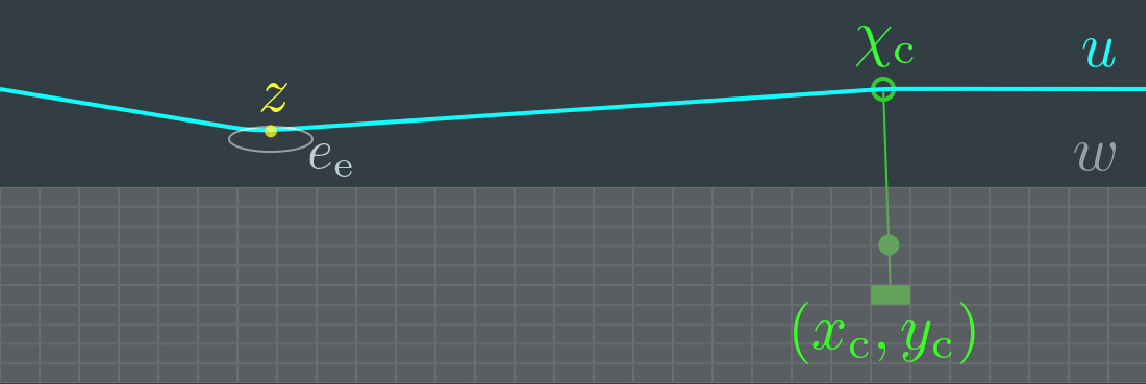
\includegraphics[width = \columnwidth]{snapshot.pdf}
    \caption{Snapshot of the application including a string and a thin plate with a connection between them. The string is excited using a pluck.}
    \label{fig:snapshot}
\end{figure}
\section{Discrete Time}

In order to implement the models described in Section \ref{sec:models} using FDTD methods, a spatio-temporal grid needs to be defined.

% One can approximate the state of a system in isolation as $q(\boldsymbol{x}, t) \approxeq q_{\boldsymbol{l}}^n$ where $q_{\boldsymbol{l}}^n$ approximates $q(\boldsymbol{x}, t)$ at time $t=nk$ with time index $n = 0, 1, 2 \hdots$ and time step $k = 1/\fs$ (in s) where $\fs$ is the sample rate (in Hz), and spatial index $\boldsymbol{l}$ depending on the system at hand. For the stiff string, space is subdivided into $N$ equal intervals of length $h_\stxt$ (in m) according to $\chi = p h_\stxt$ with spatial index $\boldsymbol{l} = p \in \{0, \hdots, N\}$. This yields the following grid function: $u(\chi, t) \approxeq u_p^n$.

% In the case of the stiff membrane, the spatial coordinate is discretised onto  as $(x, y) = (l h_\ptxt, m h_\ptxt)$ where $\boldsymbol{l} = (l,m)$ and $l \in \{0, \hdots, N_x\}$ and $m \in \{0, \hdots, N_y\}$. Here, $N_x$ and $N_y$ are the number of intervals in the $x$ and $y$ direction respectively. Notice that the same value for grid spacing $h_\ptxt$ is used for both the $x$ and $y$ directions. Using these definitions, we obtain $z(x, y, t) \approxeq z_{(l,m)}^n$.

For all models, time is discretised to $t = nk$ with time index $n = 0, 1, 2 \hdots$ and time step $k = 1/\fs$ (in s) where $\fs$ is the sample rate (in Hz). For the stiff string, space is subdivided into $N$ equal intervals of length $h_\stxt$ (in m) according to $\chi = p h$ with spatial index $p \in \{0, \hdots, N\}$. 

In the case of the stiff membrane, the spatial coordinate is discretised as $(x, y) = (l h, m h)$ where spatial indices $l \in \{0, \hdots, N_x\}$ and $m\in\{0, \hdots, N_y\}$. Here, $N_x$ and $N_y$ are the number of intervals in the $x$ and $y$ direction respectively. Notice that the same value for grid spacing $h$ is used for both the $x$ and $y$ directions. 

Using these definitions, the general state variable $q(\boldsymbol{x}, t)$ can be approximated to grid function $q_{\boldsymbol{l}}^n$, where for the stiff string $\boldsymbol{l} = p$ yielding grid function $u_p^n$ and for the stiff membrane $\boldsymbol{l} = (l, m)$ yielding grid function $z_{(l,m)}^n$.

\subsection{FDTD schemes}
The general form in Eq. \eqref{eq:generalForm} can be discretised to the following FDTD scheme:
\begin{equation}\label{eq:generalFormDisc}
    \ell q_{\boldsymbol{l}}^n = 0
\end{equation}
where $\ell$ is the discretised version of linear partial differential operator $\mathcal{L}$. Consider the following approximations to temporal derivatives:
\begin{subequations}
\begin{align}
    \ptt q&\approxeq\dtt q_{\boldsymbol{l}}^n = \frac{1}{k^2}\left(q_{\boldsymbol{l}}^{n+1} - 2 q_{\boldsymbol{l}}^n + q_{\boldsymbol{l}}^{n-1}\right),\\
    \pt q&\approxeq \dtd q_{\boldsymbol{l}}^n = \frac{1}{2k}\left(q_{\boldsymbol{l}}^{n+1} - q_{\boldsymbol{l}}^{n-1}\right),\label{eq:firstOrderCentred}\\
    \pt q&\approxeq\dtm q_{\boldsymbol{l}}^n = \frac{1}{k}\left(q_{\boldsymbol{l}}^n - q_{\boldsymbol{l}}^{n-1}\right).
\end{align}
\end{subequations}
After expansion, for any FDTD scheme, and any definition of $\ell$, one gets an update equation of the form
\begin{equation}\label{eq:generalUpdate}
    a q_{\boldsymbol{l}}^{n+1} = b q_{\boldsymbol{l}}^n + c q_{\boldsymbol{l}}^{n-1}
\end{equation}
where $a$, $b$ and $c$ depend on the system at hand. 

To illustrate, one can discretise the stiff string. Writing Eq. \eqref{eq:generalFormDisc} for the stiff string as
\begin{equation}
    \ell_\text{s} u_p^n = 0
\end{equation}
where $\ell_\stxt$ as a discrete version of Eq. \eqref{eq:stiffString}. Approximating the spatial derivatives using the following operators:
\begin{subequations}
\begin{align}
    \pcc u&\approxeq \dcc u_p^n = \frac{1}{h^2}\left(u_{p+1}^n - 2 u_p^n + u_{p-1}^n\right) \\
    \pcccc u&\approxeq \dcccc u_p^n = \dcc\dcc u_p^n
\end{align}
\end{subequations}
one can expand these, resulting in
\begin{equation}
    a_\stxt u_p^{n+1} = b_\stxt u_p^n + c_\stxt u_p^{n-1}
\end{equation}
where
\begin{equation}
\begin{aligned}
a_\stxt &= \frac{\rho A}{k^2} + \frac{\sigma_0 \rho A}{k},\\
b_\stxt &= \frac{2\rho A}{k^2} + T\dcc - EI \dcc\dcc + \frac{2\sigma_1\rho A}{k},\\
c_\stxt &= -\frac{\rho A}{k^2} +\frac{\sigma_0\rho A}{k} - \frac{2\sigma_1\rho A}{k}.
    \end{aligned}
\end{equation}
% The discrete-time definitions of Eqs. \eqref{eq:stiffString} and \eqref{eq:stiffMembrane} will not be given here for brevity, but can be found in the literature (e.g. \cite{theBible}, \cite{WillemsenThesis}). However, for any FDTD scheme, and any definition of $\ell$, one can expand \eqref{eq:generalFormDisc} to yields an update equation of the form
% \begin{equation}\label{eq:generalUpdate}
%     a q_{\boldsymbol{l}}^{n+1} = b q_{\boldsymbol{l}}^n + c q_{\boldsymbol{l}}^{n-1}
% \end{equation}
% where $a$, $b$ and $c$ depend on the system at hand. It is important to note -- for solving the connections in the next section -- that $a$ includes all variables included in the acceleration term of $\mathcal{L}$, i.e., $\rho A / k^2$ for the string and $\rho H / k^2$ for the membrane. 
Notice that these definitions are left unsimplified (e.g. dividing all terms by $\rho A / k^2$) as this is required for solving for the connection forces later on. The discrete-time definition of the stiff membrane in Eq. \eqref{eq:stiffMembrane} will not be given here for brevity, but can be found in the literature (e.g. \cite{theBible}, \cite{WillemsenThesis}).

The stability condition for the discrete models is
\begin{equation}
    h\geq \sqrt{\beta\left(c^2k^2 + 4 \sigma_1k+\sqrt{(c^2k^2 + 4 \sigma_1k)^2 + 16 \kappa^2k^2}\right)}
\end{equation}
where for the string $c^2 = T/\rho A$, $\kappa^2 = EI/\rho A$ and $\beta = 0.5$, and for the membrane $c^2 = T / \rho H$, $\kappa^2 = D/\rho H$ and $\beta = 1$. 
\subsection{Connections}\label{sec:discConnections}
% For simplicity, this work assumes the connections to be between grid points. Other work on connected FDTD schemes (see e.g. \cite{Sudholt2021}) allow for connection locations to be between grid points and use interpolation to account for this.  

To apply the effect of connections to FDTD schemes, interpolation and spreading operators must be introduced. As in Section \ref{sec:contConnections}, consider $M$ models where the grid function of the $m$\textsuperscript{th} model is $q_{m, \boldsymbol{l}_m}^n$. One can define (zeroth-order) interpolation operator
\begin{equation}
    I_{m, \boldsymbol{l}_m}(\boldsymbol{x}_m) = \begin{cases}
    1&\quad \text{if}\ \boldsymbol{l}_m= \floor[\boldsymbol{x}_m/h_m]\\
    0, &\quad\text{otherwise}
    \end{cases}
\end{equation}
and can be applied to grid function $q_{m, \boldsymbol{l}_m}^n$, to to obtain the state of one grid point of the system. A spreading operator can then be defined as
\begin{equation}\label{eq:spreading}
    J_{m, \boldsymbol{l}_m}(\boldsymbol{x}_m) = \frac{1}{(h_m)^\varepsilon}I_{m, \boldsymbol{l}_m}(\boldsymbol{x}_m),
\end{equation}
where $\varepsilon$ is the number of spatial dimensions the system is defined over ($\varepsilon = 1$ for 1D systems, $\varepsilon = 2$ for 2D systems). Equation \eqref{eq:spreading} can then be used to localise a force onto a specific location along a system. 
The general form in Eq. \eqref{eq:generalFormConnections} can be discretised to
\begin{equation}\label{eq:generalFormConnections}
    \!\!\!\ell_mq_{m, \boldsymbol{l}_m}^n =\!\sum_{\substack{c\in \mathcal{C}\vspace{0.1em}\\ r_c = m}}\!\! J_{m, \boldsymbol{l}_m}(\boldsymbol{x}_{r, c}) f_c^n-\!\! \sum_{\substack{c\in \mathcal{C}\vspace{0.1em}\\ s_c = m}}\!\! J_{m, \boldsymbol{l}_m}(\boldsymbol{x}_{s, c}) f_c^n,
\end{equation}

% where 
% \begin{equation}
%     J_{m, \boldsymbol{l},0}(\boldsymbol{x}_m) = \begin{cases}
%     \frac{1}{h_m^d}&\quad \text{if}\ \boldsymbol{l} = \floor[\boldsymbol{x}_m/h_m]\\
%     0, &\quad\text{otherwise}
%     \end{cases}
% \end{equation}
% is a spreading operator that localises the connection force of the $c$\textsuperscript{th} connection $f_c^n$ to location $\boldsymbol{x}$. Here, $d$ is the number of spatial dimensions the system is defined over ($d = 1$ for 1D systems, $d = 2$ for 2D systems). 

Assuming that none of the connections overlap one can then explicitly solve for the forces $f_c^n$. One can express the relative distance between two models ($q_{s_c}$ and $q_{r_c}$) connected by connection $c$ as
\begin{equation}\label{eq:eta}
    \eta_c^n =  I_{s_c,\boldsymbol{l}_{s_c}}(\boldsymbol{x}_{s,c})q_{s_c, \boldsymbol{l}_{s_c}}^n - I_{r_c,\boldsymbol{l}_{r_c}}(\boldsymbol{x}_{r,c})q_{r_c, \boldsymbol{l}_{r_c}}^n.
\end{equation}
If a rigid connection is chosen, the force of connection $c$ can be solved for according to
\begin{equation}\label{eq:rigidConnDisc}
    f_c^n = \frac{\eta^\star_c}{\frac{1}{a_{r_c}(h_{r_c})^{\varepsilon_{r_c}}}+ \frac{1}{a_{s_c}(h_{s_c})^{\varepsilon_{s_c}}}},
\end{equation}
where $h_m$ and $\varepsilon_m$ are the grid spacing and number of dimensions of the $m$\textsuperscript{th} model, respectively. Furthermore, 
\begin{equation}
    q_{m,\boldsymbol{l}_m}^\star = \frac{b_m q_{m,\boldsymbol{l}_m}^n + c_m q_{m,\boldsymbol{l}_m}^{n-1}}{a_m}
\end{equation}
is the state of model $q_m$ at the next time step in isolation,  i.e., without the connection forces (obtained by rewriting Eq. \eqref{eq:generalUpdate}), and can be appropriately filled into Eq. \eqref{eq:eta} to obtain $\eta_c^\star$.

Introducing the centred averaging operator
\begin{align}
    \mtd \eta^n = \frac{1}{2}\left(\eta^{n+1}+\eta^{n-1}\right)\approxeq \eta,
\end{align}
and using Eq. \eqref{eq:firstOrderCentred}, the spring in Eq. \eqref{eq:nonlinearSpring} can be discretised to
\begin{equation}\label{eq:nonlinearSpringDisc}
    f_\ctxt^n = K_{1,\ctxt}\mtd\eta_\ctxt^n + K_{3,\ctxt}(\eta_\ctxt^n)^2\mtd\eta_\ctxt^n + R_\ctxt\dtd \eta_\ctxt^n,
\end{equation}
which can be shown to be inherently stable \cite{theBible, Bilbao2009Modular}. The connection force can then be solved for according to
\begin{equation}\label{eq:springConnDisc}
    f_c^n = \frac{\eta_c^\star + \frac{\gamma_{c,-}}{\gamma_{c,+}}\eta_c^{n-1}}{\frac{1}{\gamma_{c,+}} + \frac{1}{a_{r_c}(h_{r_c})^{\varepsilon_{r_c}}}+ \frac{1}{a_{s_c}(h_{s_c})^{\varepsilon_{s_c}}}},
\end{equation}
where 
\begin{equation}
    \gamma_{c,\pm} = \frac{K_{1, c}}{2} + \frac{K_{3,c}(\eta_c^n)^2}{2} \pm \frac{R_c}{2k}.
\end{equation}
Notice that the rigid connection in Eq. \eqref{eq:rigidConnDisc} is a special case of Eq. \eqref{eq:springConnDisc} where $\eta^{n-1}_c = 0$ and $\gamma_{c, +} \rightarrow \infty$.
\subsection{Excitations}\label{sec:discExcitations}
This section discretises the excitations found in Section \ref{sec:contExcitations}. 

\subsubsection{The Bow}
The discretisation of the friction model in Eq. \eqref{eq:bowForce} as well as its implementation using an iterative solver such as Newton-Raphson is well-covered in the literature (see e.g. \cite[Ch. 8]{WillemsenThesis})
and will thus not be detailed here. 
The bow can be discretised  For the bow, 

In the application presented here, a cubic interpolator $J_{p,3}$ is used for finer control.
\begin{equation}\label{eq:cubicJ}
    J_{p,3}(\chi_\itxt) = \frac{1}{h}\begin{cases}
        -\alpha_\itxt (\alpha_\itxt-1)(\alpha_\itxt-2)/6, & p = p_\itxt-1,\\
        (\alpha_\itxt-1)(\alpha_\itxt+1)(\alpha_\itxt-2)/2,  & p = p_\itxt,\\
        -\alpha_\itxt (\alpha_\itxt+1)(\alpha_\itxt-2)/2, & p = p_\itxt + 1,\\
        \alpha_\itxt (\alpha_\itxt+1)(\alpha_\itxt-1)/6, & p = p_\itxt + 2,\\
        0, & \text{otherwise.}
    \end{cases}
\end{equation}
where $l_\itxt = \floor[\chi_\itxt / h]$ and $\alpha_\itxt = \chi_\itxt /h - l_\itxt$.

\subsubsection{Hammer and Pluck}


For the pluck, if $|J_{p, 0}(\chi_\etxt) f_\etxt| > \varphi$ where $\varphi$ is a threshold, 

Note that the force will be scaled by the grid spacing through the inclusion of $J_{p, 0}$ such that the plucking interaction will be similar for strings with different values of $h$. 

\section{Real-Time Application}

Figure \ref{fig:gui} shows the graphical user interface of the application. The application is divided into three parts: the control panel (bottom), the excitation panel (right), and the instruments / interaction area. After describing the system architecture, this section will go into detail for all three components of the application.
An extensive demo of the application, going through all of the functionality described in this section, can be found online\footnote{\url{https://youtu.be/o6I2DlFIbsc}}.
\begin{figure*}[t]
    \centering
    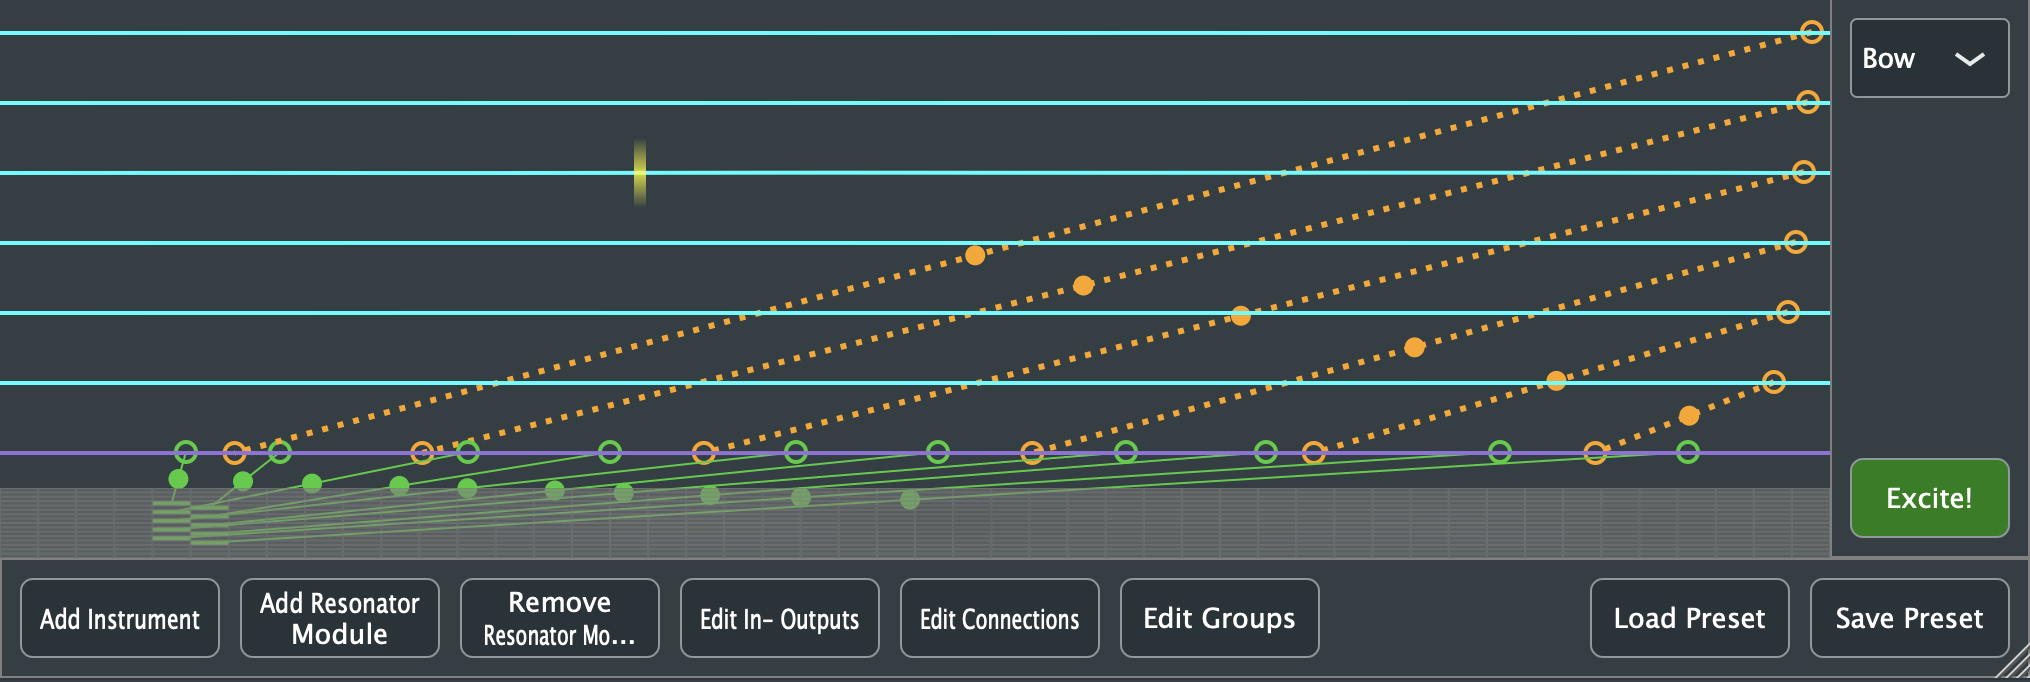
\includegraphics[width = \textwidth]{GUI.png}
    \caption{The graphical user interface (GUI) of the application. Here the guitar preset is loaded.}
    \label{fig:gui}
\end{figure*}
\subsection{System Architecture}
Figure \ref{fig:systemArchitecture} illustrates the architecture of the audio-generating part of the application.

\begin{figure}[h]
    \centering
    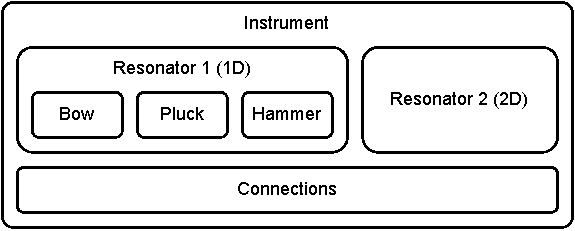
\includegraphics[width = \columnwidth]{systemArchitectureSMC2022.pdf}
    \caption{System Architecture. }
    \label{fig:systemArchitecture}
\end{figure}


The application can contain several independent instruments each of which can possess several resonators. Every 1D resonator has three exciter modules, one for each of the excitations described in this paper. Furthermore, instruments contain information about the connections between various resonators.

\subsection{Resonator modules}
The available resonators are: the stiff string, bar, membrane, thin plate and stiff membrane. 

For the stiff string and the bar an advanced and non-advanced list of parameters  
\begin{itemize}
    \item Stiff string
    \item Bar
    \item Membrane
    \item Thin Plate
    \item Stiff Membrane
\end{itemize}

\subsection{Control panel}
The control panel contains several buttons, the visibility of which is controlled by the state of the application. The main buttons are: `Add Instrument', `Add Resonator Module', `Remove Resonator Module', `Edit In- Outputs', `Edit Connections', `Edit Groups'. If any of the three latter buttons are clicked, the control panel will show instructions on how to edit the chosen option. Additional buttons are related to loading and saving presets, further elaborated on in Section \ref{sec:presets} 

For any  button is pressed states of all resonator modules will be set to 0.

Instructions will be shown... 

\subsection{Instrument area}


\subsubsection{Model Interaction}
Only 1D models can be excited

scroll wheel is linked to $-0.2 \leq v_\Btxt \leq 0.2$ if the bowing excitation is chosen. If instead the hammer or pluck interaction are chosen, the scrollwheel is linked to the excitation width $h \leq e_\text{w} \leq 10 h$. 

The direction of the bowing is visualised with a moving gradient 


\subsubsection{Modules}
The various modules a user can choose are the following
\begin{itemize}
    \item Stiff string
    \item Bar
    \item Membrane
    \item Thin Plate
    \item Stiff Membrane
\end{itemize}

2D models get an extra parameters: maxPoints, so as to not overload the CPU.

\subsubsection{Outputs}
The output of any model can be obtained by listening to $q(\boldsymbol{l}_\text{o}, t)$ for an output location $\boldsymbol{l}_\text{o}$. In the application it is possible to retrieve 

One can adjust the listening points 

Left, right and stereo channels are shown in white, red and yellow respectively. 

\subsubsection{Connections}
Rigid connections are shown in green, linear springs in orange and non-linear springs in magenta. 

Although experiments with overlapping connections have been done, it has been decided to exclude these from the application. Following \cite{Bilbao2009Modular}, although any number of overlapping connections can be explicitly calculated, one needs to do a matrix inverse every sample. Therefore, it was decided to exclude overlapping connections from the application. 


\subsubsection{Groups}
Various models can be grouped together
\subsubsection{Presets}\label{sec:presets}
\begin{itemize}
    \item Instrument 0
    \begin{itemize}
        \item Resonator 0
        \begin{itemize}
            \itemsep0em 
            \item Parameter 1
            \item Parameter 2
            \item ...
        \end{itemize}
        \item Resonator 1
        \item Resonator 2
    \end{itemize}
\end{itemize}

\subsection{Excitation}
The excitation panel contains a dropdown menu including the bow, hammer and pluck excitations.

If the hammer is triggered when the mass is further away from the string, the excitation will be of higher amplitude.

\subsection{Fixed parameters}
\begin{table}[h]\label{tab:parameters}
\begin{center}
\begin{tabular}{|l|c|c|}
    \hline
    Name & Symbol (unit) & Value\\ \hline
    \multicolumn{3}{|l|}{\bf Bow}\\ \hline
    Free parameter & $a_\Btxt$ (-) & $100$\\
    Bow force & $f_\Btxt$ (N) & $40 \cdot \rho A$\\\hline
    \multicolumn{3}{|l|}{\bf Hammer / pluck}\\ \hline
    Mass & $M_\text{z}$ (kg) & 0.01\\
    Spring coefficient & $K_\text{z}$ (N/m) & 1000\\
    Collision stiffness& $K_\etxt$ (N/m$^\alpha_\etxt$) & $10^6$\\
    Nonlin. coll. coeff. & $\alpha_\etxt$ (-) & 1.3\\\hline
    \multicolumn{3}{|l|}{\bf Connections}\\ \hline
    Linear spring coeff. & $K_1$ (N/m)  & $10^8$ \\
    Nonlin. spring coeff. & $K_3$ (N/m$^3$)  & $10^{10}$
    \\\hline
\end{tabular}
\caption{List of fixed parameter values.}
\end{center}
\end{table}
\section{Results}

\begin{table}[]
    \centering
    \begin{tabular}{|l|c|c|c|c|}
        \hline  & None & Rigid & Linear & Nonlinear \\\hline
        No graphics & 3.8 & 8.3 & 13 & 13\\
        Graphics & 12.7 & 28.4 & 42.3 & 43.1\\\hline
    \end{tabular}
    \caption{CPU usage (in \%) of two identical strings ($N=118$) with all moving grid points connected ($C = 117$) using various connection types.}
    \label{tab:CPU}
\end{table}

\section{Discussion}
To the best of the authors' knowledge, the way of real-time interactive excitation used for the hammer and the pluck has not been done before. 

% Right now, changes between sample rates are not included in the functionality of the application. As the sample rate is linked to the number of grid points, the locations of the outputs and connections are not included in the   the presets assume a sample

\section{Conclusion}

Applying excitations to 2D systems.

Port to Virtual Reality

Adding inputs so that the application can be used as an effect. 

Acoustic tubes

Exciting resonator with exciter of another (bowed tube, lip-excited string)

Pitch change


\begin{acknowledgments}
This work has been funded in part by the European Art-Science-Technology Network for Digital Creativity (EASTN-DC), project number 883023.
\end{acknowledgments} 

%%%%%%%%%%%%%%%%%%%%%%%%%%%%%%%%%%%%%%%%%%%%%%%%%%%%%%%%%%%%%%%%%%%%%%%%%%%%%
%bibliography here
\bibliography{smc2022bib}

\end{document}
